\pagebreak
\section{Describe how you have used MapReduce jobs to solve the social network problem.} \label{T4}

\paragraph{}We used MapRoduce to solve the Social Network problem. MapReduce is a technique used to divide a problem then solve in parallel using multiple machine. It divides the problem in smaller groups so it can be solved faster. The sum of all the result obtain are then all put together to obtain your the final solution.\\
\\
\begin{center}
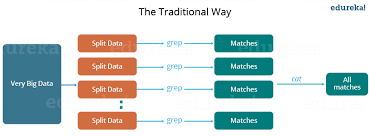
\includegraphics[width=13cm]{Resources/MapReduce.png}\\
\emph{Figure 4.1 - MapReduce on Big Data}
\end{center}
\paragraph{}In our implementation, the input is splitted in users/friends entries. These entries can then be divided in smaller groups. We process these entries in our Map function, which outputs first and second degree friends associated to each user. A reduce step is then used to process the output of the map step in order to build a set of recommendation for each user. This way, the problem can be solved in parallel on different threads/machines.